\documentclass[tikz,border=6pt]{standalone}
\usepackage{tikz}
\usepackage{fontspec}
\usepackage{xcolor}

\setsansfont[Ligatures=TeX, BoldFont={* Medium}]{Fira Sans}
\renewcommand{\familydefault}{\sfdefault}

\usetikzlibrary{positioning, arrows.meta, fit, shapes.geometric, backgrounds}

%% Colors matching Bruno theme
\definecolor{brunoblue}{HTML}{182936}
\definecolor{titlecolor}{RGB}{196,13,30}
\definecolor{brunolightgray}{HTML}{E6E6E6}
\definecolor{darkgreen}{RGB}{0,130,0}
\definecolor{lightblue}{RGB}{220,235,250}
\definecolor{lightred}{RGB}{255,230,228}
\definecolor{lightgreen}{RGB}{225,245,228}

%% Prevent hyphenation globally
\hyphenpenalty=10000
\exhyphenpenalty=10000

\begin{document}
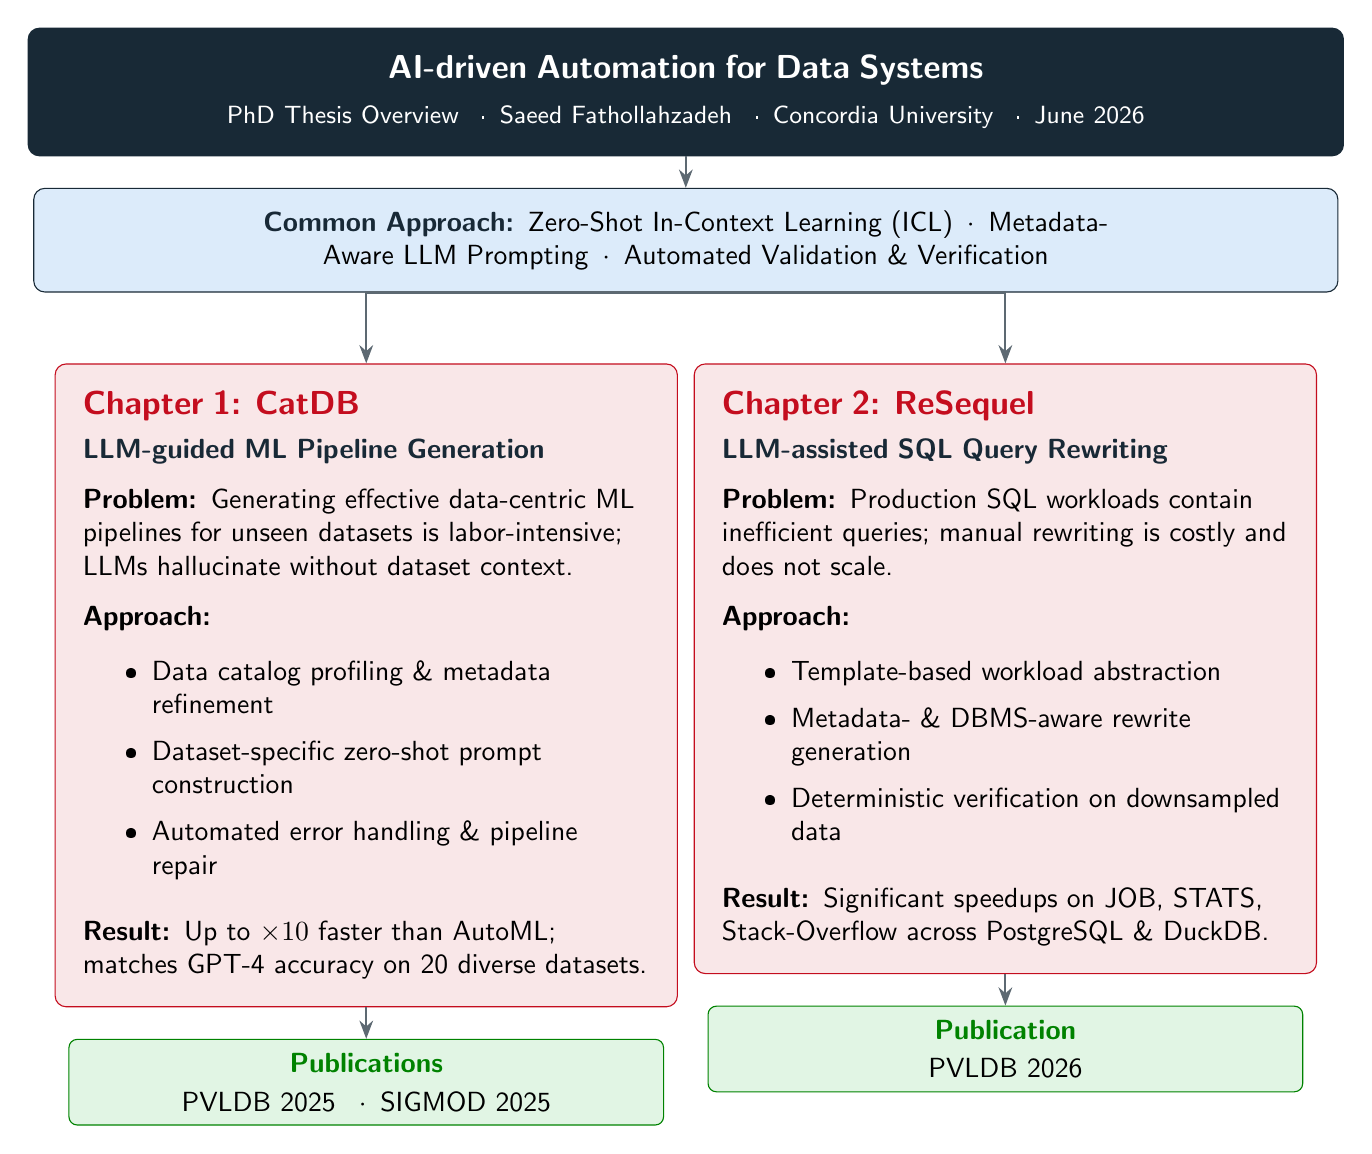
\begin{tikzpicture}[
  font=\sffamily,
  >=Stealth,
  titlebox/.style={
    draw=brunoblue, fill=brunoblue, text=white,
    rounded corners=4pt, align=center,
    inner sep=10pt, text width=#1
  },
  chapterbox/.style={
    draw=titlecolor, fill=titlecolor!10,
    rounded corners=4pt, align=left,
    inner sep=10pt, text width=#1
  },
  pubbox/.style={
    draw=darkgreen, fill=lightgreen,
    rounded corners=3pt, align=center,
    inner sep=5pt, text width=#1
  },
  arrow/.style={->, thick, color=brunoblue!70}
]

%% ─────────────────── TOP TITLE BOX ───────────────────
\node[titlebox=16cm] (title) at (0,0) {%
  {\large\bfseries AI-driven Automation for Data Systems}\\[4pt]
  {\small PhD Thesis Overview
  \enspace·\enspace Saeed Fathollahzadeh
  \enspace·\enspace Concordia University
  \enspace·\enspace June 2026}
};

%% ─────────────────── UNIFYING THEME ───────────────────
\node[draw=brunoblue, fill=lightblue, rounded corners=4pt,
      align=center, inner sep=8pt, text width=16cm,
      below=0.4cm of title] (theme) {%
  {\bfseries\color{brunoblue} Common Approach:}\enspace
  Zero-Shot In-Context Learning (ICL)\enspace$\cdot$\enspace
  Metadata-Aware LLM Prompting\enspace$\cdot$\enspace
  Automated Validation \& Verification
};

%% ─────────────── CHAPTER 1: CatDB ───────────────
\node[chapterbox=7.2cm, below left=0.9cm and 0.1cm of theme.south] (catdb) {%
  {\color{titlecolor}\bfseries\large Chapter 1: CatDB}\\[4pt]
  {\bfseries\color{brunoblue}LLM-guided ML Pipeline Generation}\\[6pt]
  \textbf{Problem:} Generating effective data-centric ML
  pipelines for unseen datasets is labor-intensive;
  LLMs hallucinate without dataset context.\\[6pt]
  \textbf{Approach:}
  \begin{itemize}\setlength\itemsep{1pt}
    \item Data catalog profiling \& metadata refinement
    \item Dataset-specific zero-shot prompt construction
    \item Automated error handling \& pipeline repair
  \end{itemize}
  \vspace{4pt}
  \textbf{Result:} Up to ${\times}10$ faster than AutoML;
  matches GPT-4 accuracy on 20 diverse datasets.
};

%% ─────────────── CHAPTER 2: ReSequel ───────────────
\node[chapterbox=7.2cm, below right=0.9cm and 0.1cm of theme.south] (resequel) {%
  {\color{titlecolor}\bfseries\large Chapter 2: ReSequel}\\[4pt]
  {\bfseries\color{brunoblue}LLM-assisted SQL Query Rewriting}\\[6pt]
  \textbf{Problem:} Production SQL workloads contain
  inefficient queries; manual rewriting is costly
  and does not scale.\\[6pt]
  \textbf{Approach:}
  \begin{itemize}\setlength\itemsep{1pt}
    \item Template-based workload abstraction
    \item Metadata- \& DBMS-aware rewrite generation
    \item Deterministic verification on downsampled data
  \end{itemize}
  \vspace{4pt}
  \textbf{Result:} Significant speedups on JOB, STATS,
  Stack-Overflow across PostgreSQL \& DuckDB.
};

%% ─────────────── PUBLICATION BADGES ───────────────
\node[pubbox=7.2cm, below=0.4cm of catdb] (catdb_pub) {%
  \textbf{\color{darkgreen}Publications}\\[2pt]
  PVLDB 2025 \enspace$\cdot$\enspace SIGMOD 2025
};

\node[pubbox=7.2cm, below=0.4cm of resequel] (resequel_pub) {%
  \textbf{\color{darkgreen}Publication}\\[2pt]
  PVLDB 2026
};

%% ─────────────── ARROWS ───────────────
\draw[arrow] (title.south) -- (theme.north);
\draw[arrow] (theme.south) -| (catdb.north);
\draw[arrow] (theme.south) -| (resequel.north);
\draw[arrow] (catdb.south) -- (catdb_pub.north);
\draw[arrow] (resequel.south) -- (resequel_pub.north);

\end{tikzpicture}
\end{document}
